\documentclass[15pt,a4paper]{article}

%use the english line for english reports
%usepackage[english]{babel}
\usepackage[portuguese]{babel}
\usepackage[utf8]{inputenc}
\usepackage{indentfirst}
\usepackage{graphicx}
\usepackage{verbatim}
\usepackage{cite}
\usepackage{url}


\begin{document}

\setlength{\textwidth}{16cm}
\setlength{\textheight}{22cm}

\title{\Large\textbf{JogginGo!}\linebreak\linebreak\linebreak
\Large\textbf{Relatório Final}\linebreak\linebreak

\includegraphics[height=6cm, width=7cm]{feup.pdf}\linebreak \linebreak
\Large{Mestrado Integrado em Engenharia Informática e Computação} \linebreak \linebreak
\Large{Paradigmas de Programação}\linebreak
}

\author{\textbf{Grupo XX:}\\ \\ Luís Dias - 080509094 - ei08094@fe.up.pt \\ Luís Gomes - 080509169 - ei08169@fe.up.pt \\\linebreak\linebreak \\
\\ Faculdade de Engenharia da Universidade do Porto \\ Rua Roberto Frias, s\/n, 4200-465 Porto, Portugal \linebreak\linebreak\linebreak
\linebreak\linebreak\vspace{1cm}}
%\date{27 de Maio de 2013}
\maketitle
\thispagestyle{empty}

%************************************************************************************************
%************************************************************************************************

\newpage

\tableofcontents

%************************************************************************************************
%************************************************************************************************

%*************************************************************************************************
%************************************************************************************************

\newpage

\section{}

\section{Introdução}

\subsection{Descrição do cenário}
Durante uma viagem, um condutor tem que tomar determinadas decisões, sob variadas influências, até chegar ao seu destino. O condutor pode pretender chegar rapidamente ao seu destino (p.e trabalho) ou preferir realizar um percurso turístico, visitanto diversos locais dispersos pela cidade. É com base nestas condições que é escolhido o melhor percurso.

No entanto, o problema o condutor não sabe \textit{à priori} os obstáculos que irá encontrar durante a sua viagem, como é natural. O caminho a percorrer seria facilmente determinado se assim fosse. Desta forma, o condutor devera ter conhecimento das adversidades à medida que, provavelmente,se deverá deparar com elas durante o seu percurso.

\subsection{Objectivo do trabalho}

O objectivo deste trabalho é implementar um agente BDI capaz de derminar o melhor percurso a realizar numa viagem dentro de uma cidade e indicá-lo ao condutor. Por outras palavras, pretende-se que o agente tenha a capacidade de recolher informações sobre o ambiente e as diferentes componentes (locais a visitar, estado meteorológico, acidentes, tempo e gasolina disponíveis) e, com base nestes, levar o condutor ao seu destino.

%\subsection{Resultados esperados e forma de avaliação}
%Após o sistema estar devidamente implementado, pretende-se que o agente seja capaz de tomar o melhor percurso, com base nas %condições definidas \textit{à priori}, como por exemplo, o tipo de rota (que pode ser directa ou turística).

%Por exemplo, se o tipo de rota escolhida for directa, pretende-se que o agente se dirija directamente do ponto de partida ao de %chegada, sem alterar o seu caminho para passar em pontos de interesse.\\ Por outro lado, se o tipo de rota escolhida for turística, %pretende-se que o agente vá do ponto de partida ao de chegada, passando pelos pontos de interesses definidos para essa rota.

\newpage
\section{Especificação}

\subsection{Identificação e caracterização dos agentes}
A aplicação contém um agente, Driver (condutor). O condutor tem como conhecimentos iniciais o ponto inicial da viagem, o destino final, e tempo e gasolina que tem para viajar. 
O agente determina qual o melhor caminho a percorrer com base no que observa ao seu redor e no tipo de viagem que está a fazer (directa para o destino final ou passando por pontos de interesse).

No caso de ter como configuração a viagem directa para o destino final, o condutor vai ignorar todos os pontos de interesse e dirigir-se directamente para o destino, escolhendo o melhor caminho possível (mais curto).
Caso opte por uma viagem turística, irá percorrer todos os pontos de interesse possiveis antes de se dirigir para o fim. Cada ponto de interesse pode ser visitado sobre determinadas condições, por exemplo o estado do tempo e se esse local já foi visitado anteriormente. A escolha do ponto de interesse a visitar é determinada como sendo a localização que tem o caminho mais curto desde a posição em que o condutor está. Depois da visita a cada um dos pontos de interesse, este é assinalado como "visitado" e é calculado o próximo melhor local a visitar.

Em ambas as configurações existem adversidades que podem influenciar e interromper o caminho a percorrer pelo condutor. Podem acontecer acidentes dos quais o condutor, naturalmente, não tinha conhecimento antes de estarem no seu campo de visão. Neste caso, o condutor tem de recalcular o caminho sabendo que aquele esta interrompido, e aqui também é feito o cálculo do melhor caminho, podendo fazer com que mude o actual ponto de interesse a visitar. Isto acontece pois não faria sentido o condutor ir ao mesmo local mesmo que passasse por um outro ponto de interesse que ficasse consideravelmente mais perto.
Outro dos factores é o tempo. O condutor tem um determinado tempo para visitar pontos de interesse (por exemplo uma manhã antes do trabalho). Caso esse tempo termine, a viagem turística do condutor é interrompida e este dirige-se para o destino final. Finalmente, o condutor pode ficar com pouca gasolina. Quando o carro atinge a reserva, o seu caminho actual é interrompido para abastecer, de forma a garantir que pode continuar a viajar sem ficar sem gasolina. Assim que abastece, verifica qual o melhor local a visitar e prossegue com a sua viagem.\\\\Para além do Agente Driver, existe a Aplicação GPSBDI. A sua função é contruir o mundo através do qual o condutor viaja e recolhe informações. A aplicação GPSBDI contém, assim, o mapa que contém todos os caminhos possíveis para o condutor,  o tempo e gasolina restantes que o condutor tem para fazer a viagem, a lista de pontos de interesse que existem no mundo, acidentes e localização dos pontos inicial e final.\\\\

\begin{figure}[htp]
  \centering
  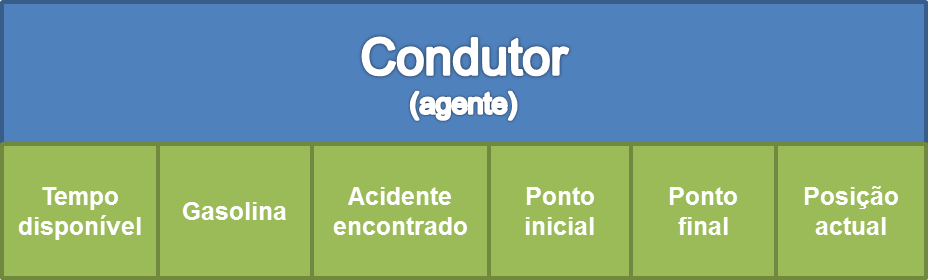
\includegraphics[scale=0.5]{diagrama_condutor.png}
  \caption{Arquitectura do agente Driver}
\end{figure}

\begin{figure}[htp]
  \centering
  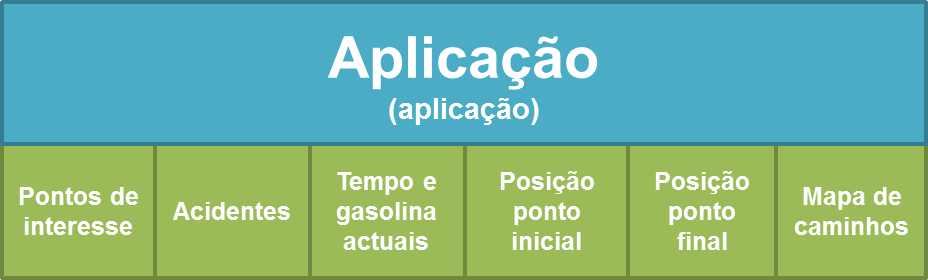
\includegraphics[scale=0.5]{diagrama_aplicacao.png}
  \caption{Arquitectura da aplicacao GPSBDI}
\end{figure}

\subsection{Protocolos de interacção}

O agente Driver (condutor) contém todos os beliefs, goals e plans necessários para interacção com o mundo exterior. Assim, a aplicação GPSBDI contém toda a informação que o condutor necessita de recolher para fazer a viagem. Esta interacção é feita através do espaço 2D (Grid2D), que contém todos os componentes presentes no mundo, desde pontos de interesse a acidentes, passando por estações de abastecimento.
Exemplo de interacção: o condutor começa, e detecta um acidente através da informação que a Aplicação lhe dá; define esse acidente como evitado e marca-o no mapa de estradas; ao mesmo tempo a aplicação actualiza o tempo e gasolina restantes do condutor, e quando este se apercebe da falta de um deles executa o plano respectivo.
Esta interacção é definida, de uma forma simples, pelo esquema abaixo.

\begin{figure}[htp]
  \centering
  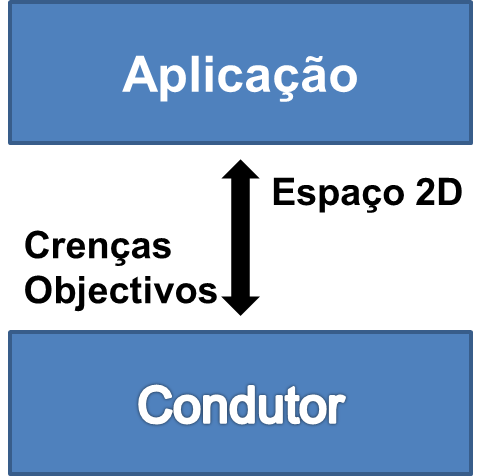
\includegraphics[scale=0.5]{diagrama_interaccao_final.png}
  \caption{Arquitectura da aplicacao GPSBDI}
\end{figure}

\newpage
\section{Desenvolvimento}

\subsection{Plataforma e ambiente de desenvolvimento}
Os agentes racionais têm uma representação explícita no ambiente e dos objetivos que estão a tentar atingir. Assim, e tal como definido no ponto anterior, o Jadex assenta numa filosofia BDI (\textit{Belief-Desire-Intention}). Mais tarde, este modelo foi transformado numa teoria um pouco mais formal, baseado em crenças, objectivos e planos (\textit{Beliefs, Goals and Plans}).

As crenças, permitem enumerar aquilo que o agente sabe antes da execução do programa. Neste caso, a localização de pontos de interesse é um exemplo de crença.
No que toca aos objectivos, as coisas já não são tão lineares. Há 4 tipos de objectivos:
\begin{itemize}
  \item \textit{Perform Goal:} Isto é algo que tem que ser feito, mas que não leva necessariamente a um resultado específico;
  \item \textit{Achieve Goal:} Representa um estado a atingir, sem especificar o caminho para lá chegar. Um agente pode tentar executar mais do que um plano para tentar chegar a este objectivo;
  \item \textit{Query Goal:} Semelhante ao \textit{Achive Goal}, no entanto não é um estado do ambiente, mas sim um estado interno. Por outras palavras, serve para recolher informações que o agente necessite;
  \item \textit{Maintain Goal:} É um objectivo que depois de atingido, é para manter.
\end{itemize}
Quanto aos planos, descrevem a forma como as acções do agente se desenrolam. Os planos são, assim, "activados" de acordo com a ocorrência de eventos (serão descritos mais à frente) e objectivos. Um dos grandes aspectos da estrutura BDI é que esta selecção é feita automaticamente.////Como IDE(\textit{Integrated development environment}) foi utilizado o Eclipse, que é uma ferramenta com a qual já temos alguma confiança e não requer aprendizagem. Para além disso, a versão mais actualizada já contém integração com projectos no Git (para controlo de versões), o que permitiu ter sempre a versão mais actualizada e funcional do projecto no IDE. Tudo isto foi utilizado em Windows 7.
 
\subsection{Estrutura da aplicação}
\subsubsection{Módulos da aplicação}

O sistema é constituído por um grande módulo principal, a Aplicação, que contém toda a informação relativa ao Jadex. Dentro da aplicação, temos a componente XML e a respectiva componente Java. Aqui temos módulos de:

\begin{itemize}

\item Contrução de mapa: BDIMap. Aqui é inicializado o mapa de estradas para o condutor percorrer, com 1 nas posições que são estrada e 0 nas restantes.
\item Movimentação: ShortestPath, GoPlanEnv e GoAction. A primeira contém o algoritmo que calcula os caminhos mais curtos - será explicada mais à frente; A segunda é relativa ao plano \textit{GoPlan} do condutor. Constitui toda a parte de escolha de caminhos com base no algoritmo; A terceira é invocada pelo \textit{goPlanEnv}, e é aqui que acontece o movimento propriamente dito, com a definição da nova posição no espaço 2D.
\item Controlo de acidentes: CheckAcident. Faz parte do plano \textit{checkAccident} do condutor, e é criado quando este encontra algum acidente e necessita de "aprender" esse acidente e recalcular o caminho.
\item Colocação de gasolina:  FillGas. É utilizado quando o condutor atinge a reserva do depósito de combustível, e é invocado quando a condição de criação do respectivo plano \textit{fillGas} é atingida. 
\end{itemize}

\subsubsection{Detalhes relevantes da implementação}

Como referimos na secção acima, existem 4 módulos principais no que toca ao funcionamento do projecto. Esses encontram-se dentro da Aplicação e, mais concretamente, divididos entre o agente Driver (\textbf{condutor}) e a aplicação GPSBDI (\textbf{mundo}).\\\\ \textbf{Driver:}
\begin{itemize}
\item Beliefs:
\subitem - env: Espaço onde se encontra o agente;
\subitem - myself: O próprio agente enquanto objecto representado no espaço;
\subitem - pos: Actual posição no mundo;
\subitem - time: tempo que tem disponível para fazer a sua viagem;
\subitem - gas: gasolina que tem disponível para fazer a sua viagem;
\subitem - reserva: limite mínimo de combustível para o agente saber que tem de abastecer;
\subitem - acidente: ultimo acidente encontrado pelo condutor, e informa-o que tem de recalcular o caminho.
\item Goals:
\subitem - check: é invocado quando o condutor encontra algum acidente, e lança o plano CheckAccident ao mesmo tempo que interrompe o goal actual;
\subitem - fill: inicia quando o combustível atinge o valor da reserva, lançando o plano FillGas ao mesmo tempo que interrompe o goal actual;
\subitem - go: é o goal principal, responsável por levar o condutor até ao ponto de interesse actual/destino final. Lança o plano GoPlanEnv.
\item Plans:
\subitem - CheckAccident: É accionado quando o goal check é iniciado, e é responsável por "aprender" o acidente, assinalando-o no mapa de estradas e informando o condutor que pode recalcular o caminho.
\subitem - FillGas: Inicia assim que é criado o goal fill, e é responsável por levar o condutor a abastecer no posto de combustível mais próximo.
\subitem - GoPlanEnv: Plano principal, responsável por guiar o agente condutor para o seu próximo destino. É aqui também que verifica se, depois de visitar um local, tem tempo para visitar outro ou se tem de se dirigir para o destino final.\\\\
\end{itemize}

\textbf{GPSBDI:}
\begin{itemize}
\item Objectos:
\subitem - driver: objecto do tipo do agente Driver, contém os valores de tempo, combustível, etc.;
\subitem - accident: objecto que representa um acidente, e contém o seu estado (evitado/não evitado);
\subitem - homebase/final Destination: objectos que representam a posição inicial/final do percurso;
\subitem - pointofinterest: representa um ponto de interesse, assim como as suas caracteristicas;
\subitem - gas\_station: representa um ponto de combustível, sendo possivel definir com que valor é que este abastece o carro;
\subitem - cell: representa um bloco de estrada, isto é, um conjunto de cells representa as estradas.
\item Processos:
\subitem - BDImap: processo que inicializa o mapa de estradas representado no mundo.
\item Agentes:
\subitem - Driver: único agente do sistema, que é o condutor que viaja no mundo.\\
\end{itemize}


\textbf{Determinação de percurso mais curto}

Para encontrar qual o melhor caminho para o ponto de interesse a visitar, foi necessário recorrer a um algoritmo que nos desse exactamente isso. Assim, foi implementado o algoritmo A*, com base, entre outros, no pseudo-código encontrado na Wikipédia (ver referências). Assim, para uma matriz de caminhos, o algoritmo define o caminho mais curto entre um par de nós.\\

\textbf{Movimento do condutor}

Para o agente se movimentar entre duas posições, depois de saber se há caminho entre estas, é utilizada uma \textit{action} (GoAction) que desloca o condutor para a proxima posição. A direcção é definida determinando se o próximo nó se encontra no mesmo eixo vertical e/ou horizontal, sendo assim possível definir se vai para cima, baixo, esquerda ou direita. De seguida é actualizada a posição do condutor para a nova posição calculada.\\


Determinação da direcção e invocação da GoAction:
\begin{verbatim}

							int md= 0;
							if(mypos.getYAsInteger() == next.y){ //HORIZONTAL
								if(mypos.getXAsInteger() < next.x)
									md = 1; // DIREITA
								else if(mypos.getXAsInteger() > next.x)
									md = -1; //ESQUERDA
							}
							else
								md = 0;


							switch(md){
							case 1:
								dir = GoAction.RIGHT;
								break;
							case -1:
								dir = GoAction.LEFT;
								break;
							default:
								if(mypos.getXAsInteger() == next.x){
									if(mypos.getYAsInteger() < next.y) 
										md = 1; //BAIXO
									else if(mypos.getYAsInteger() > next.y)
										md = -1; //CIMA
								}
								switch(md){
								case 1:
									dir = GoAction.DOWN;
									break;
								case -1:
									dir = GoAction.UP;
								}
							}



							//Inform what is the new direction and execute space action
							Map params = new HashMap();
							params.put(GoAction.DIRECTION, dir);
							params.put(ISpaceAction.OBJECT_ID, env.getAvatar(getComponentDescription()).getId());
							SyncResultListener srl	= new SyncResultListener();
							env.performSpaceAction("go", params, srl); 
							srl.waitForResult();
\end{verbatim}

\newpage

Acção GoAction, responsável por actualizar a posição do condutor:

\begin{verbatim}
String dir = (String)parameters.get(DIRECTION);
		Object oid = parameters.get(ISpaceAction.OBJECT_ID);
		ISpaceObject obj = space.getSpaceObject(oid);
		IVector2 pos = (IVector2)obj.getProperty(Space2D.PROPERTY_POSITION);
		
		int px = pos.getXAsInteger();
		int py = pos.getYAsInteger();
		
		switch(dir){
		case UP:
			pos = new Vector2Int(px, py-1);
			break;
		case DOWN:
			pos = new Vector2Int(px, py+1);
			break;
		case LEFT:
			pos = new Vector2Int(px-1, py);
			break;
		case RIGHT:
			pos = new Vector2Int(px+1, py);
			break;
		}
	
		((Space2D)space).setPosition(oid, pos);
		obj.setProperty("lastmove", dir);
\end{verbatim}


\textbf{Determinação do próximo ponto de interesse a visitar}

Para saber qual o ponto de interesse mais próximo, é percorrida a lista de pontos de interesse e as suas posições, e para cada um dos destinos é calculada a distância mais curta. De seguida, é assinalada como próxima vista a que for melhor (mais perto). De referir que para cada visita é verificado se o condutor tem tempo para a visitar. Caso não tenha, vai para o destino final. Da mesma forma, determina-se se ainda há localizações por visitar. Se não houverem mais, o condutor dirige-se para o final.

\begin{verbatim}

HashMap <Integer,ISpaceObject> shorter = new HashMap <Integer,ISpaceObject>();

			/*verificar próxima visita, que será a mais próxima do ponto inicial*/
			for(int x=0; x < locations.length; x++){
				if(locations[x].getProperty("status").equals("notvisited") &&
						(locations[x].getProperty("weather").equals("")||
						 locations[x].getProperty("weather").equals((String)env.getProperty("weather"))
						 ) 
				  ){

					IVector2 actual = (IVector2)locations[x].getProperty("position");

					List<Node> nodes = GetPath((IVector2) myself.getProperty(Space2D.PROPERTY_POSITION),actual);

					if(nodes != null)
						shorter.put(nodes.size(),locations[x]);					
				}
			}

			List ll = new LinkedList(); // Collections.sort() recebe como parametro um list  
			ll.addAll(shorter.keySet());// buscando os valores no Map  
			Collections.sort(ll);

			ISpaceObject next_visit = null;

			//verifica se anda tem pontos para visitar
			if(!ll.isEmpty()){

				ISpaceObject aux = (ISpaceObject)shorter.get(ll.get(0));
				IVector2 posicao = (IVector2)aux.getProperty("position");

				//Caminho entre o ponto de interesse a visitar
				//e o destino
				List<Node> nodes = GetPath(posicao, target);
				
				//total = distancia até ao ponto de interesse + distância do ponto de interesse até ao final
				int total = nodes.size()+(Integer)ll.get(0);
				
				
				/*verificação do tempo, caso tenha tempo visita a melhor,
				 * senão vai para o desino final*/
				if((Integer)myself.getProperty("time") >= total){
					next_visit = (ISpaceObject)shorter.get(ll.get(0));
					myself.setProperty("time", (Integer)myself.getProperty("time")-total);
				}
				else{
					next_visit = fd;
					System.out.println("Fiquei sem tempo, tenho de ir para o destino final");
				}
			}
			else 
				next_visit = fd;

\end{verbatim}

\newpage
\section{Experiências}
\subsection{Objectivo de cada experiência}
Foram realizadas experiências nas duas configurações existentes (Visita Turística e Directa). Ambas as dimensões têm um mapa igual, com dimensões de 22x22, um ponto inicial, um final, acidentes, pontos de interesse e pontos de abastecimento de combustível. Para isso, utilizámos o algoritmo A* para calcular o melhor caminho entre o ponto em que o condutor se encontra, até ao próximo ponto de interesse a visita. É esse algoritmo que informa o condutor qual o ponto de interesse mais próximo da posição actual.

\begin{figure}[htp]
  \centering
  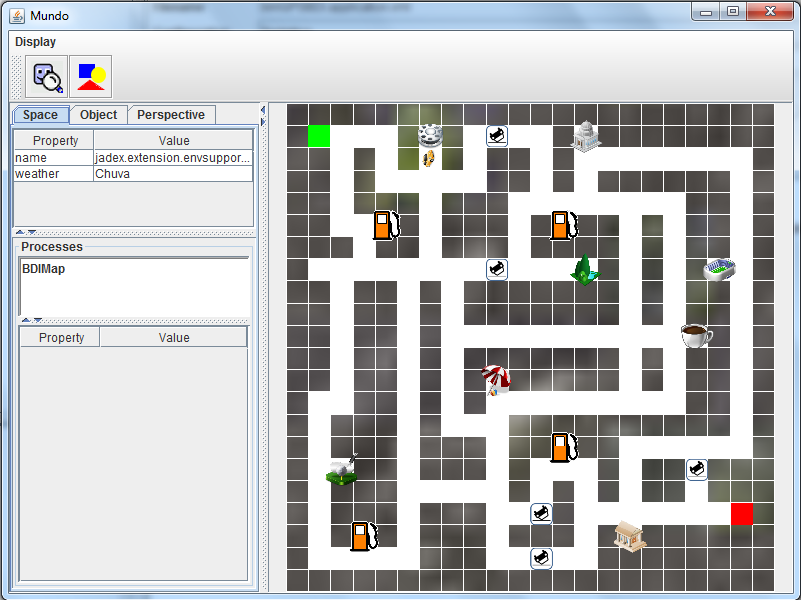
\includegraphics[scale=0.5]{mapa_mundo.png}
  \caption{Interface de simulação}
\end{figure}

\begin{figure}[htp]
  \centering
  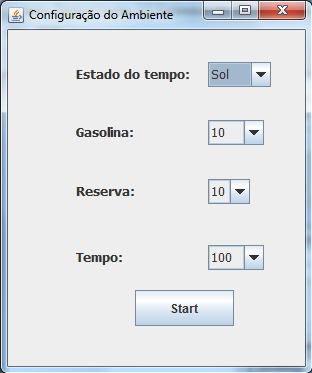
\includegraphics[scale=0.6]{launch_config.png}
  \caption{Interface de parametrização}
\end{figure}

\subsection{Visita Turística}
Nesta configuração, o condutor tem que, partindo do ponto inicial, chegar ao ponto final, passando por todos os pontos de interesse. No entanto, a ida a esse pontos de interesse, irá variar mediante estarem reunidas, ou não, as condições necessárias. 

\subsubsection{Condições atmosférias}
Certos pontos de interesse só podem ser visitados se uma determinada condição atmosférias se verificar. Por exemplo, o condutor só visita o ponto de interesse \textit{beach} (praia) se a condição atmosférias for "Sol". Da mesma maneira que o condutor apenas se desloca ao cinema se estiver "Chuva".

\subsubsection{Tempo}
A visita de todos os pontos de interesse, também está dependente do tempo que o condutor tiver disponível. Por outras palavras, o condutor só visita determinado ponto de interesse, se o tempo que demorar até lá, e de lá ao ponto final, for menor do que o tempo que este ainda tem disponível, caso contrário, dirigir-se-á directamente para o ponto final. Esta verificação é feita em cada deslocação para um ponto de interesse.

\subsubsection{Gasolina}
O condutor tem definido um campo "reserva". É este valor que dita o momento em que o condutor procura um posto de abastecimento. Para além disso, é necessário referir que cada posto de abastecimento tem um campo "gas" definidio, que indica a quantia que esse posto de abastecimento fornece ao condutor.

\subsubsection{Acidentes}
Quando o condutor encontra um acidente, recalcula o caminho. No entanto, pode alterar o destino. Isto é, se o condutor estiver para o campo de golf, e encontrar um acidente, volta a chamar o algoritmo de cálculo de caminhos. Neste passo, pode verificar que existe um ponto de interesse mais próximo, do que o novo caminho que precisaria para continuar em direcção ao capo de golf. Quando isto acontece, o condutor altera o seu ponto de interesse de destino.

\subsection{Directo}
Nesta configuração, o condutor dirige-se imediatamente para o ponto final, sem visitar qualquer ponto de interesse. No entanto, restrições relacionadas com o combustível ou acidentes, são também verificadas.

\subsection{Resultados}
Todas as experiências acima referidas, se verificaram um sucesso, visto que o condutor respeitou as condições por nós definidas no momento da execução do programa, tomando as decisões acertadas para cada um dos casos. Estamos em posição de afirmar que o comportamento do condutor foi exactamente o esperado, para os diferentes cenários testados.

\newpage
\section{Conclusões}
O objectivo deste trabalho passou pela implementação de um agente BDI capaz de aconselhar um condutor sobre as decisões a tomar, quando este se encontra na estrada. Procurámos implementar restrições de maneira a que o problema se aproximasse o máximo possível da realidade. Daí termos implementado funcionalidades como valor do combustível ou reserva.

Como mostrado ao longo deste relatório, implementámos uma interface gráfica de maneira a facilitar a definição dos valores iniciais ao utilizador. Ou seja, permitimos que o utilizador defina o valor de combustível, reserva, tempo disponível e a condição atmosférica.


A principal componente e prioridade na realização deste sistema era a capacidade de informar um agente condutor do caminho mais curto para um determinado percurso. Este objectivo foi realizado, e para além disto ainda fomos capazes de adicionar condicionantes e factores que alteram o comportamento do agente em tempo real. Neste aspecto ficamos satisfeitos por verificar que o sistema final era mais realista em termos de acontecimentos do que inicialmente planeado.

Este projecto tornou-se bastante enriquecedor para o grupo já que permitiu ter como produto final um sistema que consideramos bastante realista e que se enquadra bastante bem no conceito BDI e na alteração de comportamentos em tempo real. O agente a qualquer momento pode deparar-se com algum factor que lance uma nova intenção, estando sempre pronto para reconhecer alterações no mundo exterior.

Como maiores dificuldades, consideramos a fase inicial de aprendizagem da arquitectura BDI, já que foi bastante difícil conseguir passar para o Jadex as ideias que queríamos implementar. No entanto, com alguma pesquisa e utilização de exemplos de sistemas parecidos fomos capazes de desenvolver o produto final com bastante aproveitamento.

\newpage
\section{Melhoramentos}

Tendo em conta o tempo que foi utilizado na aprendizagem da ferramenta, o tempo disponível não permitiu ter a aplicação final completamente de acordo com o que seria ideal.

Como principal melhoramento, gostariamos de ter implementado mais funcionalidades na interface gráfica que permissem, em tempo real, adicionar acidentes/pontos de interesse ao mundo, ou até postos de combustível.

Também teria sido bastante positivo termos um sistema multi-agente, com mais condutores e a existência de eventos que permitissem trocar mensagens entre eles, avisando-os, por exemplo, que encontraram um acidente numa determinada posição ou até que foram visitar um local mas que este se encontrava encerrado.

\newpage
\section{Recursos}

\subsection{Bibliografia}

\begin{itemize}
\item Jadex, \emph{http://jadex-agents.informatik.uni-hamburg.de}, Dezembro 2012
\item Agentes e Inteligência Artificial Distribuída, \emph{http://paginas.fe.up.pt/~eol/AIAD/aiad1112.html}, Dezembro 2012
\item Jadex BDI Agent System (Soundforge), \emph{http://sourceforge.net/projects/jadex/}, Dezembro 2012
\item A\* search Algorithm, \emph{http://en.wikipedia.org/wiki/A*\_search\_algorithm}, Dezembro 2012 
\item A-Star Algorithm in Java, \emph{http://memoization.com/2008/11/30/a-star-algorithm-in-java}, Dezembro 2012
\end{itemize}

\subsection{Software}

\begin{itemize}
\item Eclipse - IDE utilizado para desenvolvimento.
\item Jadex 2.0
\item TeXworks - utilizado para a escrita do relatório em LaTeX
\end{itemize}

\subsection{Elementos do Grupo}

\begin{itemize}
\item Luís Carlos Moreira Dias, 080509094 - 50\%
\item Luís Filipe Castanheira Gomes, 080509094 - 50\%
\end{itemize}

\newpage
\appendix
\section{Apêndice}
\subsection{Manual de Utilização}
Aquando do lançamento do projecto através do IDE Eclipse, é apresentada a seguinte janela:

\begin{figure}[htp]
  \centering
  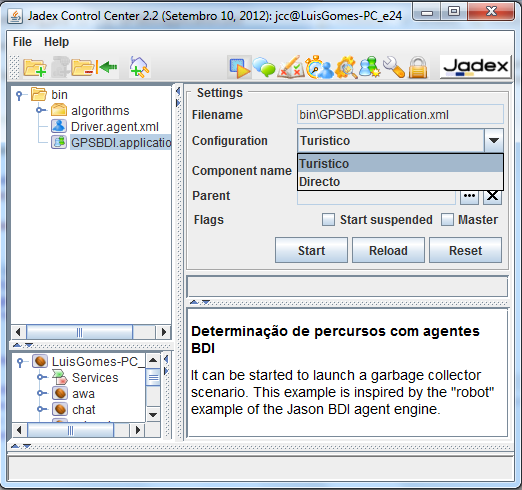
\includegraphics {configuration_choose.png}
  \caption{Interface de parametrização}
\end{figure}
Aqui podemos escolher qual a configuração pretendida. Se queremos uma Visita Turística, passando pelos pontos de interesse, ou se pretendemos navegar directamente para o ponto final. 
Após escolhida e carregado o botão "Start" deparamos com a seguinte interface:

\begin{figure}[htp]
  \centering
  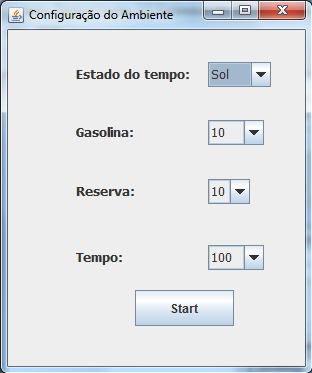
\includegraphics[scale=0.5] {launch_config.png}
  \caption{Escolha da configuraçao pretendida}
\end{figure}

Nesta inferface podemos escolher os parâmetros de arranque do navegador. Podemos definir os valores da gasolina inicial, da reserva, do tempo disponível para navegação e a condição atmosférica.
De seguida, e carregando no botão "Start", o condutor começará a sua navegação.

\begin{figure}[htp]
  \centering
  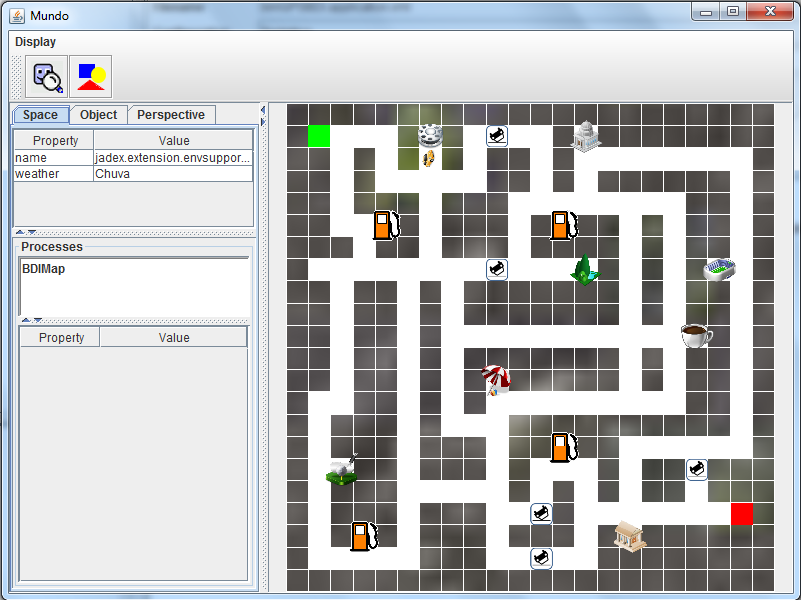
\includegraphics[scale=0.7] {mapa_mundo.png}
  \caption{Interface de parametrização}
\end{figure}

\end{document}